\section{Introduction}


\subsection{Problem Statement}
The project will investigate how to...

There is a lot of language out there :) (incl. several hundred gigabytes of Dutch, and terabytes of English \cite{buck2014n})

\subsection{Prior Work}
\label{sec:prior_work}
Since the introduction of word2vec~\cite{mikolov2013efficient, mikolov2013distributed} in 2013, the algorithm has seen a wide variety of usecases. In the initial paper~\cite{mikolov2013efficient}, Mikolov et. al describe interesting relations between vectors corresponding to words. 
A famous example of how word2vec models relations between words as mathematical equations is $king - man + woman = queen$.
The sematic relationships between man/woman and king/queen are preserved in the transformation of words to vectors, and can be expressed with basic algebra.

Subsequent papers have improved the algorithm both in terms of accuracy (\cite{levy2014linguistic}), performance, parallelization and extended the initial scope of applications. A good example of the latter is a paper by Boycheva~\cite{boycheva2015distributional}, which uses word2vec not inside the natural language processing domain but to generate playlists. Based on a set of playlists, their word2vec-based algorithm can suggest new playlists with artists that go well together.

One of the applications of word2vec, is in exploiting similarities in languages for assistance in machine translation~\cite{wolf2014joint}. Mikolov et al.~\cite{mikolov2013exploiting} released a subsequent paper on word2vec, in which they describe similarities between models of different languages. An example they give, is how the usage of the numbers one to five in English is very similar to the usage in Spanish, and likewise for the names of animals. Figure~\ref{fig:english_spanish} shows a graphical representation of word vectors in English and Spanish.

\begin{figure}[ht!]
  \centering 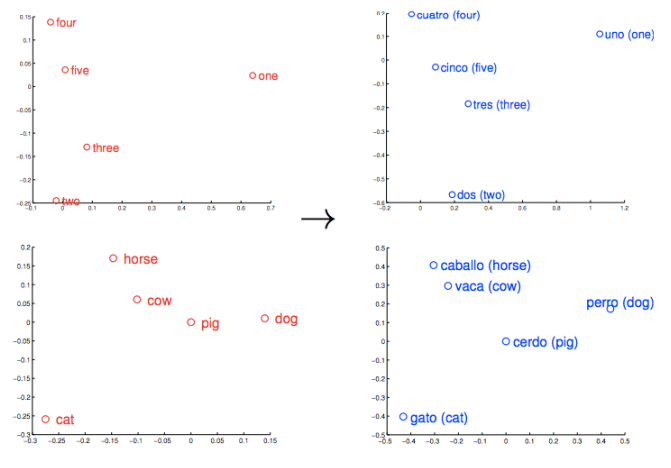
\includegraphics[width=\linewidth]{images/english_spanish}
  \caption{Vector representations of English and Spanish words, after dimensionality reduction and rotation. Notice the high level of similarity between both languages. Reprinted from Mikolov et al.~\cite{mikolov2013exploiting}}
  \label{fig:english_spanish}
\end{figure}

The similarities between languages can be used to predict translations for words without any human interaction or labeled input data. Using only unsupervised machine learning techniques, a computer could learn how to translate English to Spanish or vice versa. The only requirement is a large amount of text in both languages to train the word2vec models on.

In this research, we will focus on this specific application of word2vec: using similarities in languages to provide translations of words.

It is important to note that word2vec only uses information of cooccurrences to model words. It does not learn grammatical concepts other than by statistical analysis. This limits our translation to single words; although the translator might be able to translate each word individually, it cannot learn that each finite verb must has a subject, that "we" is plural, etc. It will learn that "swim" is to "swimming" as "walk" is to "walking", but will not know that "swimming" is a gerund.

\subsection{Research Purpose}
This research aims to improve the capabilities of machines to learn translations with minimal human intervention. Previous research~\cite{mikolov2013exploiting, wolf2014joint} has already shown potential for word2vec in the context of automatic translation, as discussed in section~\ref{sec:prior_work}.

However, we found no practical implementations using Word2Vec and no further research on different setups for word2vec based machine translation.

\section{Research goal}
The goal of this research is to give practical advice on a setup for word2vec based machine translation.

Because we aim at a practical purpose of our research, we will also release all code used in our experiments. We hope this makes our research so trivially reproducible that others will further develop and use our results.

\subsection{Tasks}
To build a test system and perform our experiments, we need to execute the following steps:

\begin{itemize}
  \item Build (at least) two working setups for automated translation:
    \begin{itemize}
      \item A single-model setup:
      \begin{itemize}
        \item Merge datasets, train single model with plain word2vec (easy)
        \item Build a translator on top of the model using the same relational structure as in the man/woman king/queen example.
      \end{itemize}
      \item A multi-model setup:
      \begin{itemize}
        \item Train the individual models
        \item Train transformation matrix between models, for example using linear regression.
        \item Build a translator that converts a word to a vector, "translates" the vector and looks up the corresponding word in the other model.
      \end{itemize}
    \end{itemize}
  \item Make a verification mechanism
  \item Verify which setup works better
\end{itemize}

\section{Planning}
A global overview of the milestones we defined in our research is as follows;
\begin{description}
  \item \emph{Half September - October: Literary Study)}\\
    During this phase, a list of relevant papers (e.g. \cite{levy2014linguistic, mikolov2013exploiting, wolf2014joint}) is collected, short-listed to a readable size and read. Each paper will get a brief (informal) summarization to capture the essence of the paper insofar as it is relevant to this research. These summaries help process the information and provide quick access during the practical research.\\

    Not all papers relevant to the research will be read during this phase, so next phases will include a fair share of reading.
  \item \emph{October: Preparing experiments}\\
    In this phase, we gather the required corpora (see Section~\ref{sec:resources}) and implement our translation programs.
  \item \emph{November: Running experiments}\\
    Running the experiments includes training the models (which might take several days) and running the translation programs against a set of predefined correct translations.
  \item \emph{Before 12 December: Incorporating results in paper}\\
    During this phase, we will incorporate the results obtained in the experiments into our final paper.
\end{description}

\section{Allocation of Responsibilities}
Marc pledges to provide sufficient beer. Bram will take care of coffee and possibly some Club-Maté.

\todo{write some actual stuff here}

\section{Resources}
\label{sec:resources}
We have identified four main resources needed for this research: a large English corpus, a large Dutch corpus, a large set of word translations from Dutch to English and computional resources to analyze the data.

The corpora for both languages should be several tens of gigabytes or more. Mikolov et al.~\cite{mikolov2013distributed} specifically state that a large amount of training data is crucial for word2vec to build a correct model. They speak of corpora 30 billion words, with a significant decrease in quality of the results when lowering the corpus size to only 6 billion words.

For this research, we will look at the following corpora:
\begin{itemize}
  \item \textit{Reddit corpus}
    \footnote{\url{https://archive.org/details/2015_reddit_comments_corpus}}
    (1TB uncompressed JSON, 50 billion words) Corpus containing all posts on Reddit. It is mostly English, but also contains a few other languages.
  \item \textit{Wikipedia EN crawl} 
    \footnote{\url{https://dumps.wikimedia.org/enwiki/20150901/}}
    (60GB uncompressed XML, 3 billion words) Corpus of all text on the English Wikipedia (ignoring revisions).
  \item \textit{Wikipedia NL Crawl} 
    \footnote{\url{https://dumps.wikimedia.org/nlwiki/20150901/}}
    (5GB uncompressed XML, 250 million words) Corpus of all text on the Dutch Wikipedia (ignoring revisions).
  \item \textit{SoNaR-500} 
    \footnote{\url{http://tst-centrale.org/producten/corpora/sonar-corpus/6-85}}
    (60GB uncompressed text, >500 million words) Curated corpus gathered by several Dutch universities, consisting of newspapers, subtitles, etc.
  \item \textit{Dutch Parallel Corpus} 
    \footnote{\url{http://tst-centrale.org/producten/corpora/dutch-parallel-corpus-niet-commercieel/6-65}}
    (10 million pairs of words Dutch-English.
\end{itemize}

These datasets are all open for academic usage, in various degrees of opennes. The Reddit corpus is available through their API or with bittorrent, the Wikipedia data is freely available for download under CC-BY-SA license, and SoNaR-500 is available after signing a special research license agreement.

Before processing the corpora with word2vec, we will convert them to a universal format: plain text, with special characters (everything that is not alphanumeric, space or dash) removed, and one entity (post, article or article) per line.

To make our research reproducable, we will publish all our code online and provide lists with hashes of all our input and intermediate steps (e.g. after cleaning the data).